\documentclass[twoside]{book}

% Packages required by doxygen
\usepackage{fixltx2e}
\usepackage{calc}
\usepackage{doxygen}
\usepackage[export]{adjustbox} % also loads graphicx
\usepackage{graphicx}
\usepackage[utf8]{inputenc}
\usepackage{makeidx}
\usepackage{multicol}
\usepackage{multirow}
\PassOptionsToPackage{warn}{textcomp}
\usepackage{textcomp}
\usepackage[nointegrals]{wasysym}
\usepackage[table]{xcolor}

% Font selection
\usepackage[T1]{fontenc}
\usepackage[scaled=.90]{helvet}
\usepackage{courier}
\usepackage{amssymb}
\usepackage{sectsty}
\renewcommand{\familydefault}{\sfdefault}
\allsectionsfont{%
  \fontseries{bc}\selectfont%
  \color{darkgray}%
}
\renewcommand{\DoxyLabelFont}{%
  \fontseries{bc}\selectfont%
  \color{darkgray}%
}
\newcommand{\+}{\discretionary{\mbox{\scriptsize$\hookleftarrow$}}{}{}}

% Page & text layout
\usepackage{geometry}
\geometry{%
  a4paper,%
  top=2.5cm,%
  bottom=2.5cm,%
  left=2.5cm,%
  right=2.5cm%
}
\tolerance=750
\hfuzz=15pt
\hbadness=750
\setlength{\emergencystretch}{15pt}
\setlength{\parindent}{0cm}
\setlength{\parskip}{3ex plus 2ex minus 2ex}
\makeatletter
\renewcommand{\paragraph}{%
  \@startsection{paragraph}{4}{0ex}{-1.0ex}{1.0ex}{%
    \normalfont\normalsize\bfseries\SS@parafont%
  }%
}
\renewcommand{\subparagraph}{%
  \@startsection{subparagraph}{5}{0ex}{-1.0ex}{1.0ex}{%
    \normalfont\normalsize\bfseries\SS@subparafont%
  }%
}
\makeatother

% Headers & footers
\usepackage{fancyhdr}
\pagestyle{fancyplain}
\fancyhead[LE]{\fancyplain{}{\bfseries\thepage}}
\fancyhead[CE]{\fancyplain{}{}}
\fancyhead[RE]{\fancyplain{}{\bfseries\leftmark}}
\fancyhead[LO]{\fancyplain{}{\bfseries\rightmark}}
\fancyhead[CO]{\fancyplain{}{}}
\fancyhead[RO]{\fancyplain{}{\bfseries\thepage}}
\fancyfoot[LE]{\fancyplain{}{}}
\fancyfoot[CE]{\fancyplain{}{}}
\fancyfoot[RE]{\fancyplain{}{\bfseries\scriptsize Generated by Doxygen }}
\fancyfoot[LO]{\fancyplain{}{\bfseries\scriptsize Generated by Doxygen }}
\fancyfoot[CO]{\fancyplain{}{}}
\fancyfoot[RO]{\fancyplain{}{}}
\renewcommand{\footrulewidth}{0.4pt}
\renewcommand{\chaptermark}[1]{%
  \markboth{#1}{}%
}
\renewcommand{\sectionmark}[1]{%
  \markright{\thesection\ #1}%
}

% Indices & bibliography
\usepackage{natbib}
\usepackage[titles]{tocloft}
\setcounter{tocdepth}{3}
\setcounter{secnumdepth}{5}
\makeindex

% Hyperlinks (required, but should be loaded last)
\usepackage{ifpdf}
\ifpdf
  \usepackage[pdftex,pagebackref=true]{hyperref}
\else
  \usepackage[ps2pdf,pagebackref=true]{hyperref}
\fi
\hypersetup{%
  colorlinks=true,%
  linkcolor=blue,%
  citecolor=blue,%
  unicode%
}

% Custom commands
\newcommand{\clearemptydoublepage}{%
  \newpage{\pagestyle{empty}\cleardoublepage}%
}

\usepackage{caption}
\captionsetup{labelsep=space,justification=centering,font={bf},singlelinecheck=off,skip=4pt,position=top}

%===== C O N T E N T S =====

\begin{document}

% Titlepage & ToC
\hypersetup{pageanchor=false,
             bookmarksnumbered=true,
             pdfencoding=unicode
            }
\pagenumbering{roman}
\begin{titlepage}
\vspace*{7cm}
\begin{center}%
{\Large Yathzee }\\
\vspace*{1cm}
{\large Generated by Doxygen 1.8.11}\\
\end{center}
\end{titlepage}
\clearemptydoublepage
\tableofcontents
\clearemptydoublepage
\pagenumbering{arabic}
\hypersetup{pageanchor=true}

%--- Begin generated contents ---
\chapter{Namespace Index}
\section{Packages}
Here are the packages with brief descriptions (if available)\+:\begin{DoxyCompactList}
\item\contentsline{section}{\hyperlink{namespace_yathzee}{Yathzee} }{\pageref{namespace_yathzee}}{}
\end{DoxyCompactList}

\chapter{Hierarchical Index}
\section{Class Hierarchy}
This inheritance list is sorted roughly, but not completely, alphabetically\+:\begin{DoxyCompactList}
\item \contentsline{section}{Yathzee.\+Dice\+Generator}{\pageref{class_yathzee_1_1_dice_generator}}{}
\item \contentsline{section}{Yathzee.\+Die}{\pageref{class_yathzee_1_1_die}}{}
\item \contentsline{section}{Yathzee.\+Die\+Image}{\pageref{class_yathzee_1_1_die_image}}{}
\item Form\begin{DoxyCompactList}
\item \contentsline{section}{Yathzee.\+Form1}{\pageref{class_yathzee_1_1_form1}}{}
\end{DoxyCompactList}
\item \contentsline{section}{Yathzee.\+Score\+Section}{\pageref{class_yathzee_1_1_score_section}}{}
\begin{DoxyCompactList}
\item \contentsline{section}{Yathzee.\+Lower\+Score\+Section}{\pageref{class_yathzee_1_1_lower_score_section}}{}
\item \contentsline{section}{Yathzee.\+Upper\+Score\+Section}{\pageref{class_yathzee_1_1_upper_score_section}}{}
\end{DoxyCompactList}
\end{DoxyCompactList}

\chapter{Class Index}
\section{Class List}
Here are the classes, structs, unions and interfaces with brief descriptions\+:\begin{DoxyCompactList}
\item\contentsline{section}{\hyperlink{class_yathzee_1_1_dice_generator}{Yathzee.\+Dice\+Generator} \\*Class responsible for creating \hyperlink{class_yathzee_1_1_die}{Die} objects. }{\pageref{class_yathzee_1_1_dice_generator}}{}
\item\contentsline{section}{\hyperlink{class_yathzee_1_1_die}{Yathzee.\+Die} \\*\hyperlink{class_yathzee_1_1_die}{Die} objects are objects that have a die value, and a \hyperlink{class_yathzee_1_1_die_image}{Die\+Image} }{\pageref{class_yathzee_1_1_die}}{}
\item\contentsline{section}{\hyperlink{class_yathzee_1_1_die_image}{Yathzee.\+Die\+Image} }{\pageref{class_yathzee_1_1_die_image}}{}
\item\contentsline{section}{\hyperlink{class_yathzee_1_1_form1}{Yathzee.\+Form1} }{\pageref{class_yathzee_1_1_form1}}{}
\item\contentsline{section}{\hyperlink{class_yathzee_1_1_lower_score_section}{Yathzee.\+Lower\+Score\+Section} \\*Class responsible to hold the data for the lower score section and test the \hyperlink{class_yathzee_1_1_die}{Die} values for specific scores. }{\pageref{class_yathzee_1_1_lower_score_section}}{}
\item\contentsline{section}{\hyperlink{class_yathzee_1_1_score_section}{Yathzee.\+Score\+Section} \\*Abstract class for score section. }{\pageref{class_yathzee_1_1_score_section}}{}
\item\contentsline{section}{\hyperlink{class_yathzee_1_1_upper_score_section}{Yathzee.\+Upper\+Score\+Section} }{\pageref{class_yathzee_1_1_upper_score_section}}{}
\end{DoxyCompactList}

\chapter{Namespace Documentation}
\hypertarget{namespace_yathzee}{}\section{Yathzee Namespace Reference}
\label{namespace_yathzee}\index{Yathzee@{Yathzee}}
\subsection*{Classes}
\begin{DoxyCompactItemize}
\item 
class \hyperlink{class_yathzee_1_1_dice_generator}{Dice\+Generator}
\begin{DoxyCompactList}\small\item\em Class responsible for creating \hyperlink{class_yathzee_1_1_die}{Die} objects. \end{DoxyCompactList}\item 
class \hyperlink{class_yathzee_1_1_die}{Die}
\begin{DoxyCompactList}\small\item\em \hyperlink{class_yathzee_1_1_die}{Die} objects are objects that have a die value, and a \hyperlink{class_yathzee_1_1_die_image}{Die\+Image} \end{DoxyCompactList}\item 
class \hyperlink{class_yathzee_1_1_die_image}{Die\+Image}
\begin{DoxyCompactList}\small\item\em Gets the proper image for a die value. \end{DoxyCompactList}\item 
class \hyperlink{class_yathzee_1_1_form1}{Form1}
\begin{DoxyCompactList}\small\item\em The Graphical User Interface for \hyperlink{namespace_yathzee}{Yathzee}. \end{DoxyCompactList}\item 
class \hyperlink{class_yathzee_1_1_lower_score_section}{Lower\+Score\+Section}
\begin{DoxyCompactList}\small\item\em Class responsible to hold the data for the lower score section and test the \hyperlink{class_yathzee_1_1_die}{Die} values for specific scores. \end{DoxyCompactList}\item 
class {\bfseries Program}
\item 
class \hyperlink{class_yathzee_1_1_score_section}{Score\+Section}
\begin{DoxyCompactList}\small\item\em Abstract class for score section. \end{DoxyCompactList}\item 
class \hyperlink{class_yathzee_1_1_upper_score_section}{Upper\+Score\+Section}
\begin{DoxyCompactList}\small\item\em Class responsible to hold the data for the upper score section and test the \hyperlink{class_yathzee_1_1_die}{Die} values for specific scores. \end{DoxyCompactList}\end{DoxyCompactItemize}
\subsection*{Enumerations}
\begin{DoxyCompactItemize}
\item 
enum \hyperlink{namespace_yathzee_af9eae2784d7776b80bb77da141a63b7f}{Score\+Type\+Upper} \+: byte \{ \\*
{\bfseries One}, 
{\bfseries Two}, 
{\bfseries Three}, 
{\bfseries Four}, 
\\*
{\bfseries Five}, 
{\bfseries Six}, 
{\bfseries Bonus}, 
{\bfseries Total}
 \}\begin{DoxyCompactList}\small\item\em Score type for the upper part of the score section. \end{DoxyCompactList}
\item 
enum \hyperlink{namespace_yathzee_ae036ce06cdf75e284ea1cd78a457ef70}{Score\+Type\+Lower} \+: byte \{ \\*
{\bfseries Three\+Of\+Kind}, 
{\bfseries Four\+Of\+Kind}, 
{\bfseries Full\+House}, 
{\bfseries Small\+Straight}, 
\\*
{\bfseries Large\+Straight}, 
{\bfseries Yathzee}, 
{\bfseries Chance}, 
{\bfseries Total}
 \}\begin{DoxyCompactList}\small\item\em Score type for the lower part of the score section. \end{DoxyCompactList}
\end{DoxyCompactItemize}


\subsection{Enumeration Type Documentation}
\index{Yathzee@{Yathzee}!Score\+Type\+Lower@{Score\+Type\+Lower}}
\index{Score\+Type\+Lower@{Score\+Type\+Lower}!Yathzee@{Yathzee}}
\subsubsection[{\texorpdfstring{Score\+Type\+Lower}{ScoreTypeLower}}]{\setlength{\rightskip}{0pt plus 5cm}enum {\bf Yathzee.\+Score\+Type\+Lower} \+: byte\hspace{0.3cm}{\ttfamily [strong]}}\hypertarget{namespace_yathzee_ae036ce06cdf75e284ea1cd78a457ef70}{}\label{namespace_yathzee_ae036ce06cdf75e284ea1cd78a457ef70}


Score type for the lower part of the score section. 

\index{Yathzee@{Yathzee}!Score\+Type\+Upper@{Score\+Type\+Upper}}
\index{Score\+Type\+Upper@{Score\+Type\+Upper}!Yathzee@{Yathzee}}
\subsubsection[{\texorpdfstring{Score\+Type\+Upper}{ScoreTypeUpper}}]{\setlength{\rightskip}{0pt plus 5cm}enum {\bf Yathzee.\+Score\+Type\+Upper} \+: byte\hspace{0.3cm}{\ttfamily [strong]}}\hypertarget{namespace_yathzee_af9eae2784d7776b80bb77da141a63b7f}{}\label{namespace_yathzee_af9eae2784d7776b80bb77da141a63b7f}


Score type for the upper part of the score section. 


\chapter{Class Documentation}
\hypertarget{class_yathzee_1_1_dice_generator}{}\section{Yathzee.\+Dice\+Generator Class Reference}
\label{class_yathzee_1_1_dice_generator}\index{Yathzee.\+Dice\+Generator@{Yathzee.\+Dice\+Generator}}


Class responsible for creating \hyperlink{class_yathzee_1_1_die}{Die} objects.  


\subsection*{Public Member Functions}
\begin{DoxyCompactItemize}
\item 
\hyperlink{class_yathzee_1_1_die}{Die} \hyperlink{class_yathzee_1_1_dice_generator_aa767803e7adbf0958fb15b431f571914}{generate\+Dice} ()
\begin{DoxyCompactList}\small\item\em Creates a \hyperlink{class_yathzee_1_1_die}{Die} object using a random number generator. \end{DoxyCompactList}\end{DoxyCompactItemize}


\subsection{Detailed Description}
Class responsible for creating \hyperlink{class_yathzee_1_1_die}{Die} objects. 



\subsection{Member Function Documentation}
\index{Yathzee\+::\+Dice\+Generator@{Yathzee\+::\+Dice\+Generator}!generate\+Dice@{generate\+Dice}}
\index{generate\+Dice@{generate\+Dice}!Yathzee\+::\+Dice\+Generator@{Yathzee\+::\+Dice\+Generator}}
\subsubsection[{\texorpdfstring{generate\+Dice()}{generateDice()}}]{\setlength{\rightskip}{0pt plus 5cm}{\bf Die} Yathzee.\+Dice\+Generator.\+generate\+Dice (
\begin{DoxyParamCaption}
{}
\end{DoxyParamCaption}
)}\hypertarget{class_yathzee_1_1_dice_generator_aa767803e7adbf0958fb15b431f571914}{}\label{class_yathzee_1_1_dice_generator_aa767803e7adbf0958fb15b431f571914}


Creates a \hyperlink{class_yathzee_1_1_die}{Die} object using a random number generator. 

\begin{DoxyReturn}{Returns}
A \hyperlink{class_yathzee_1_1_die}{Die} object.
\end{DoxyReturn}


The documentation for this class was generated from the following file\+:\begin{DoxyCompactItemize}
\item 
src/\+Yathzee/Dice\+Generator.\+cs\end{DoxyCompactItemize}

\hypertarget{class_yathzee_1_1_die}{}\section{Yathzee.\+Die Class Reference}
\label{class_yathzee_1_1_die}\index{Yathzee.\+Die@{Yathzee.\+Die}}


\hyperlink{class_yathzee_1_1_die}{Die} objects are objects that have a die value, and a \hyperlink{class_yathzee_1_1_die_image}{Die\+Image}  


\subsection*{Public Member Functions}
\begin{DoxyCompactItemize}
\item 
{\bfseries Die} (int value)\hypertarget{class_yathzee_1_1_die_afc6338fb4ec4ae9b874ceb7d23331665}{}\label{class_yathzee_1_1_die_afc6338fb4ec4ae9b874ceb7d23331665}

\item 
void \hyperlink{class_yathzee_1_1_die_a7b34d8689fa88e1f25269818636fe75c}{set\+Die} (int value)
\begin{DoxyCompactList}\small\item\em Initializes the \hyperlink{class_yathzee_1_1_die}{Die} object. Sets a \hyperlink{class_yathzee_1_1_die_image}{Die\+Image} based on parameter value. \end{DoxyCompactList}\end{DoxyCompactItemize}
\subsection*{Properties}
\begin{DoxyCompactItemize}
\item 
int {\bfseries Value}\hspace{0.3cm}{\ttfamily  \mbox{[}get\mbox{]}}\hypertarget{class_yathzee_1_1_die_af7e17dadd808bcd0c4ba0d1b14ff4a9c}{}\label{class_yathzee_1_1_die_af7e17dadd808bcd0c4ba0d1b14ff4a9c}

\item 
System.\+Drawing.\+Image {\bfseries Image}\hspace{0.3cm}{\ttfamily  \mbox{[}get\mbox{]}}\hypertarget{class_yathzee_1_1_die_ad589565a256b35774112e726b700be53}{}\label{class_yathzee_1_1_die_ad589565a256b35774112e726b700be53}

\end{DoxyCompactItemize}


\subsection{Detailed Description}
\hyperlink{class_yathzee_1_1_die}{Die} objects are objects that have a die value, and a \hyperlink{class_yathzee_1_1_die_image}{Die\+Image} 



\subsection{Member Function Documentation}
\index{Yathzee\+::\+Die@{Yathzee\+::\+Die}!set\+Die@{set\+Die}}
\index{set\+Die@{set\+Die}!Yathzee\+::\+Die@{Yathzee\+::\+Die}}
\subsubsection[{\texorpdfstring{set\+Die(int value)}{setDie(int value)}}]{\setlength{\rightskip}{0pt plus 5cm}void Yathzee.\+Die.\+set\+Die (
\begin{DoxyParamCaption}
\item[{int}]{value}
\end{DoxyParamCaption}
)}\hypertarget{class_yathzee_1_1_die_a7b34d8689fa88e1f25269818636fe75c}{}\label{class_yathzee_1_1_die_a7b34d8689fa88e1f25269818636fe75c}


Initializes the \hyperlink{class_yathzee_1_1_die}{Die} object. Sets a \hyperlink{class_yathzee_1_1_die_image}{Die\+Image} based on parameter value. 


\begin{DoxyParams}{Parameters}
{\em value} & The value of the \hyperlink{class_yathzee_1_1_die}{Die} object to be set.\\
\hline
\end{DoxyParams}


The documentation for this class was generated from the following file\+:\begin{DoxyCompactItemize}
\item 
src/\+Yathzee/Die.\+cs\end{DoxyCompactItemize}

\hypertarget{class_yathzee_1_1_die_image}{}\section{Yathzee.\+Die\+Image Class Reference}
\label{class_yathzee_1_1_die_image}\index{Yathzee.\+Die\+Image@{Yathzee.\+Die\+Image}}
\subsection*{Public Member Functions}
\begin{DoxyCompactItemize}
\item 
System.\+Drawing.\+Image {\bfseries get\+Die1} ()\hypertarget{class_yathzee_1_1_die_image_a2724ca8f7897a55ffe997ef924394c7e}{}\label{class_yathzee_1_1_die_image_a2724ca8f7897a55ffe997ef924394c7e}

\item 
System.\+Drawing.\+Image {\bfseries get\+Die2} ()\hypertarget{class_yathzee_1_1_die_image_a263559c79673dcfaaed6e32611c52804}{}\label{class_yathzee_1_1_die_image_a263559c79673dcfaaed6e32611c52804}

\item 
System.\+Drawing.\+Image {\bfseries get\+Die3} ()\hypertarget{class_yathzee_1_1_die_image_ad1a3e766145e9b4866088a0774bfa30a}{}\label{class_yathzee_1_1_die_image_ad1a3e766145e9b4866088a0774bfa30a}

\item 
System.\+Drawing.\+Image {\bfseries get\+Die4} ()\hypertarget{class_yathzee_1_1_die_image_a413e19c90b843b4c1ea7a4b4eba824db}{}\label{class_yathzee_1_1_die_image_a413e19c90b843b4c1ea7a4b4eba824db}

\item 
System.\+Drawing.\+Image {\bfseries get\+Die5} ()\hypertarget{class_yathzee_1_1_die_image_a8195f245d22a93c8b57244fbb7721db2}{}\label{class_yathzee_1_1_die_image_a8195f245d22a93c8b57244fbb7721db2}

\item 
System.\+Drawing.\+Image {\bfseries get\+Die6} ()\hypertarget{class_yathzee_1_1_die_image_a320bc5d43dd0400443cfce5d81f57adb}{}\label{class_yathzee_1_1_die_image_a320bc5d43dd0400443cfce5d81f57adb}

\item 
System.\+Drawing.\+Image {\bfseries get\+Die\+Blank} ()\hypertarget{class_yathzee_1_1_die_image_a86d428cf3935a1785df461b2fa710d8f}{}\label{class_yathzee_1_1_die_image_a86d428cf3935a1785df461b2fa710d8f}

\end{DoxyCompactItemize}


The documentation for this class was generated from the following file\+:\begin{DoxyCompactItemize}
\item 
src/\+Yathzee/Die\+Image.\+cs\end{DoxyCompactItemize}

\hypertarget{class_yathzee_1_1_form1}{}\section{Yathzee.\+Form1 Class Reference}
\label{class_yathzee_1_1_form1}\index{Yathzee.\+Form1@{Yathzee.\+Form1}}
Inheritance diagram for Yathzee.\+Form1\+:\begin{figure}[H]
\begin{center}
\leavevmode
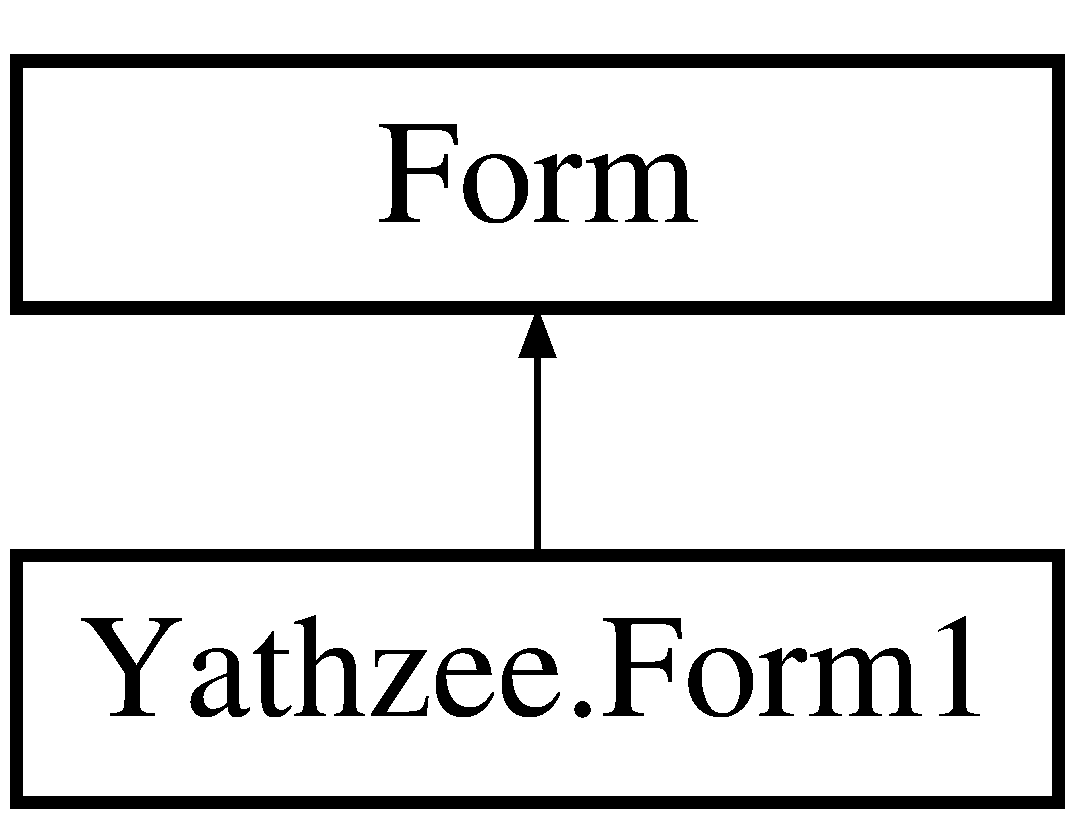
\includegraphics[height=2.000000cm]{class_yathzee_1_1_form1}
\end{center}
\end{figure}
\subsection*{Public Member Functions}
\begin{DoxyCompactItemize}
\item 
\hyperlink{class_yathzee_1_1_form1_a72fd0c431a8f1bbfae37f57917046763}{Form1} ()
\begin{DoxyCompactList}\small\item\em Sets up the G\+UI. \end{DoxyCompactList}\end{DoxyCompactItemize}
\subsection*{Protected Member Functions}
\begin{DoxyCompactItemize}
\item 
override void \hyperlink{class_yathzee_1_1_form1_a481d2704c1eb9c036cd9389d3dd866cb}{Dispose} (bool disposing)
\begin{DoxyCompactList}\small\item\em Clean up any resources being used. \end{DoxyCompactList}\end{DoxyCompactItemize}


\subsection{Constructor \& Destructor Documentation}
\index{Yathzee\+::\+Form1@{Yathzee\+::\+Form1}!Form1@{Form1}}
\index{Form1@{Form1}!Yathzee\+::\+Form1@{Yathzee\+::\+Form1}}
\subsubsection[{\texorpdfstring{Form1()}{Form1()}}]{\setlength{\rightskip}{0pt plus 5cm}Yathzee.\+Form1.\+Form1 (
\begin{DoxyParamCaption}
{}
\end{DoxyParamCaption}
)}\hypertarget{class_yathzee_1_1_form1_a72fd0c431a8f1bbfae37f57917046763}{}\label{class_yathzee_1_1_form1_a72fd0c431a8f1bbfae37f57917046763}


Sets up the G\+UI. 



\subsection{Member Function Documentation}
\index{Yathzee\+::\+Form1@{Yathzee\+::\+Form1}!Dispose@{Dispose}}
\index{Dispose@{Dispose}!Yathzee\+::\+Form1@{Yathzee\+::\+Form1}}
\subsubsection[{\texorpdfstring{Dispose(bool disposing)}{Dispose(bool disposing)}}]{\setlength{\rightskip}{0pt plus 5cm}override void Yathzee.\+Form1.\+Dispose (
\begin{DoxyParamCaption}
\item[{bool}]{disposing}
\end{DoxyParamCaption}
)\hspace{0.3cm}{\ttfamily [protected]}}\hypertarget{class_yathzee_1_1_form1_a481d2704c1eb9c036cd9389d3dd866cb}{}\label{class_yathzee_1_1_form1_a481d2704c1eb9c036cd9389d3dd866cb}


Clean up any resources being used. 


\begin{DoxyParams}{Parameters}
{\em disposing} & true if managed resources should be disposed; otherwise, false.\\
\hline
\end{DoxyParams}


The documentation for this class was generated from the following files\+:\begin{DoxyCompactItemize}
\item 
src/\+Yathzee/Form1.\+cs\item 
src/\+Yathzee/Form1.\+Designer.\+cs\end{DoxyCompactItemize}

\hypertarget{class_yathzee_1_1_lower_score_section}{}\section{Yathzee.\+Lower\+Score\+Section Class Reference}
\label{class_yathzee_1_1_lower_score_section}\index{Yathzee.\+Lower\+Score\+Section@{Yathzee.\+Lower\+Score\+Section}}
Inheritance diagram for Yathzee.\+Lower\+Score\+Section\+:\begin{figure}[H]
\begin{center}
\leavevmode
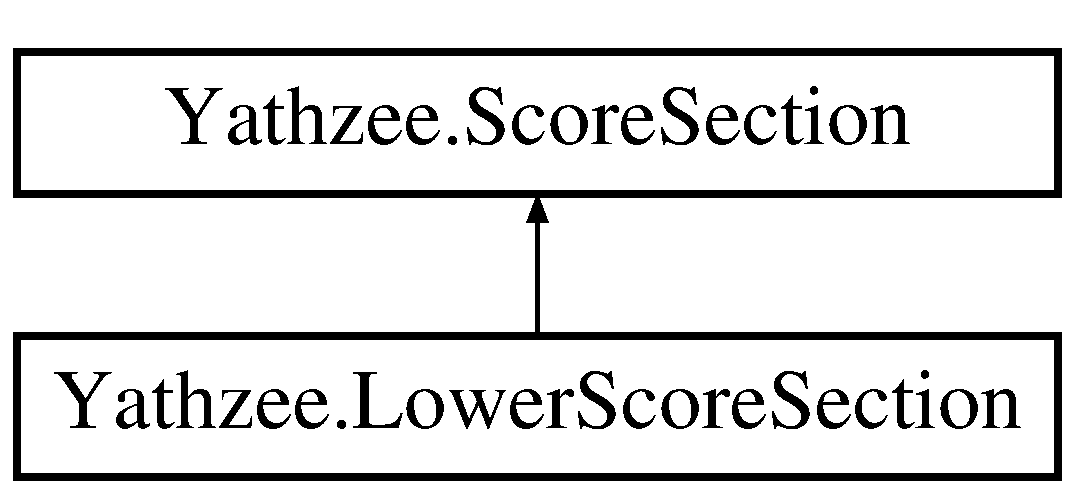
\includegraphics[height=2.000000cm]{class_yathzee_1_1_lower_score_section}
\end{center}
\end{figure}
\subsection*{Public Member Functions}
\begin{DoxyCompactItemize}
\item 
Dictionary$<$ Score\+Type\+Lower, int $>$ {\bfseries get\+Scores} ()\hypertarget{class_yathzee_1_1_lower_score_section_a427d65a33219f4e2d4965cc56f18e1a6}{}\label{class_yathzee_1_1_lower_score_section_a427d65a33219f4e2d4965cc56f18e1a6}

\item 
void {\bfseries check\+Score} (\hyperlink{class_yathzee_1_1_die}{Die}\mbox{[}$\,$\mbox{]} dice, Score\+Type\+Lower score\+Type)\hypertarget{class_yathzee_1_1_lower_score_section_acd14498c43eb2c788e450269095a9b61}{}\label{class_yathzee_1_1_lower_score_section_acd14498c43eb2c788e450269095a9b61}

\end{DoxyCompactItemize}
\subsection*{Additional Inherited Members}


The documentation for this class was generated from the following file\+:\begin{DoxyCompactItemize}
\item 
src/\+Yathzee/Lower\+Score\+Section.\+cs\end{DoxyCompactItemize}

\hypertarget{class_yathzee_1_1_score_section}{}\section{Yathzee.\+Score\+Section Class Reference}
\label{class_yathzee_1_1_score_section}\index{Yathzee.\+Score\+Section@{Yathzee.\+Score\+Section}}
Inheritance diagram for Yathzee.\+Score\+Section\+:\begin{figure}[H]
\begin{center}
\leavevmode
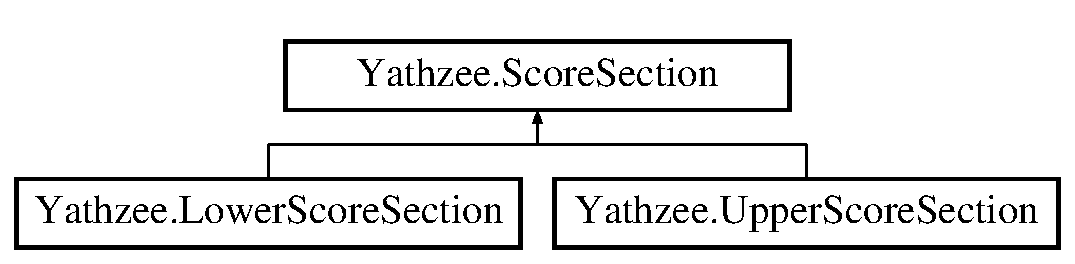
\includegraphics[height=2.000000cm]{class_yathzee_1_1_score_section}
\end{center}
\end{figure}
\subsection*{Properties}
\begin{DoxyCompactItemize}
\item 
int {\bfseries Total}\hspace{0.3cm}{\ttfamily  \mbox{[}get, set\mbox{]}}\hypertarget{class_yathzee_1_1_score_section_a58581bbdd2cda719e5f1dcd7659c412f}{}\label{class_yathzee_1_1_score_section_a58581bbdd2cda719e5f1dcd7659c412f}

\end{DoxyCompactItemize}


The documentation for this class was generated from the following file\+:\begin{DoxyCompactItemize}
\item 
src/\+Yathzee/Score\+Section.\+cs\end{DoxyCompactItemize}

\hypertarget{class_yathzee_1_1_upper_score_section}{}\section{Yathzee.\+Upper\+Score\+Section Class Reference}
\label{class_yathzee_1_1_upper_score_section}\index{Yathzee.\+Upper\+Score\+Section@{Yathzee.\+Upper\+Score\+Section}}


Class responsible to hold the data for the upper score section and test the \hyperlink{class_yathzee_1_1_die}{Die} values for specific scores.  


Inheritance diagram for Yathzee.\+Upper\+Score\+Section\+:\begin{figure}[H]
\begin{center}
\leavevmode
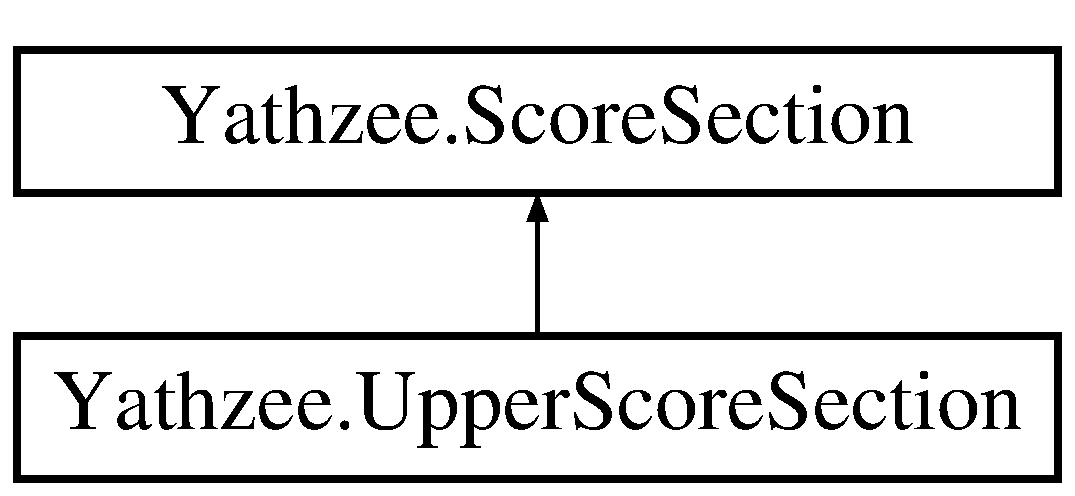
\includegraphics[height=2.000000cm]{class_yathzee_1_1_upper_score_section}
\end{center}
\end{figure}
\subsection*{Public Member Functions}
\begin{DoxyCompactItemize}
\item 
Dictionary$<$ \hyperlink{namespace_yathzee_af9eae2784d7776b80bb77da141a63b7f}{Score\+Type\+Upper}, int $>$ {\bfseries get\+Scores} ()\hypertarget{class_yathzee_1_1_upper_score_section_aa10b4b6d4c7038e80c9d221bfb482b72}{}\label{class_yathzee_1_1_upper_score_section_aa10b4b6d4c7038e80c9d221bfb482b72}

\item 
void \hyperlink{class_yathzee_1_1_upper_score_section_ae2db6ea707243900dc1b87cdc4ff9e2f}{check\+Score} (\hyperlink{class_yathzee_1_1_die}{Die}\mbox{[}$\,$\mbox{]} dice, int checked\+Value)
\begin{DoxyCompactList}\small\item\em Main entry point for the class. Checkes what the score is for a dice array with a score type, and stores it in the score\+Values Dictonary. \end{DoxyCompactList}\item 
bool \hyperlink{class_yathzee_1_1_upper_score_section_ab539f23446aface95d748a3ebc5396d2}{are\+All\+Set} ()
\begin{DoxyCompactList}\small\item\em Checks if all scores on the upper section are set. \end{DoxyCompactList}\end{DoxyCompactItemize}
\subsection*{Additional Inherited Members}


\subsection{Detailed Description}
Class responsible to hold the data for the upper score section and test the \hyperlink{class_yathzee_1_1_die}{Die} values for specific scores. 



\subsection{Member Function Documentation}
\index{Yathzee\+::\+Upper\+Score\+Section@{Yathzee\+::\+Upper\+Score\+Section}!are\+All\+Set@{are\+All\+Set}}
\index{are\+All\+Set@{are\+All\+Set}!Yathzee\+::\+Upper\+Score\+Section@{Yathzee\+::\+Upper\+Score\+Section}}
\subsubsection[{\texorpdfstring{are\+All\+Set()}{areAllSet()}}]{\setlength{\rightskip}{0pt plus 5cm}bool Yathzee.\+Upper\+Score\+Section.\+are\+All\+Set (
\begin{DoxyParamCaption}
{}
\end{DoxyParamCaption}
)}\hypertarget{class_yathzee_1_1_upper_score_section_ab539f23446aface95d748a3ebc5396d2}{}\label{class_yathzee_1_1_upper_score_section_ab539f23446aface95d748a3ebc5396d2}


Checks if all scores on the upper section are set. 

\begin{DoxyReturn}{Returns}
The result of the test.
\end{DoxyReturn}
\index{Yathzee\+::\+Upper\+Score\+Section@{Yathzee\+::\+Upper\+Score\+Section}!check\+Score@{check\+Score}}
\index{check\+Score@{check\+Score}!Yathzee\+::\+Upper\+Score\+Section@{Yathzee\+::\+Upper\+Score\+Section}}
\subsubsection[{\texorpdfstring{check\+Score(\+Die[] dice, int checked\+Value)}{checkScore(Die[] dice, int checkedValue)}}]{\setlength{\rightskip}{0pt plus 5cm}void Yathzee.\+Upper\+Score\+Section.\+check\+Score (
\begin{DoxyParamCaption}
\item[{{\bf Die}\mbox{[}$\,$\mbox{]}}]{dice, }
\item[{int}]{checked\+Value}
\end{DoxyParamCaption}
)}\hypertarget{class_yathzee_1_1_upper_score_section_ae2db6ea707243900dc1b87cdc4ff9e2f}{}\label{class_yathzee_1_1_upper_score_section_ae2db6ea707243900dc1b87cdc4ff9e2f}


Main entry point for the class. Checkes what the score is for a dice array with a score type, and stores it in the score\+Values Dictonary. 


\begin{DoxyParams}{Parameters}
{\em dice} & The array of \hyperlink{class_yathzee_1_1_die}{Die} objects to check\\
\hline
{\em score\+Type} & The score type to check against.\\
\hline
\end{DoxyParams}


The documentation for this class was generated from the following file\+:\begin{DoxyCompactItemize}
\item 
src/\+Yathzee/Upper\+Score\+Section.\+cs\end{DoxyCompactItemize}

%--- End generated contents ---

% Index
\backmatter
\newpage
\phantomsection
\clearemptydoublepage
\addcontentsline{toc}{chapter}{Index}
\printindex

\end{document}
